\newthought{Estimation} is the field of statistics that deals with the inference of some unknown variable from uncertain observations of this variable. It can be simply described by an example. Given a pair of variables $X$ and $Y$, and a model for their relationship, say $Y = aX + b\eta$, where $\eta$ is a normally distributed random variable, we could infer the value of $X$ from observations of $Y$. Using Bayes' rule we can write
\[
P(X|Y) = \frac{P(X)P(Y|X)}{P(Y)},
\]
where one can naturally deduce that $P(Y|X) = \mathcal{N}(aX,b^2)$. Assuming some prior knowledge about $X$ and that subsequent observations of $Y$ are independent and identically distributed we obtain an estimate for the value of $X$ given the experimental setup. If we are concerned with temporal processes, say a random process $X_t$ which needs to be inferred from observations of a dependent process $Y_t$ a different terminology is used. When we are interested in inferring $X_t$ from data $\{Y_s\},\,s \in [0,T]$, the problem gets named according to the value of $t$. If $t \in [0,T]$, we call this a \emph{smoothing} problem. If $t = T$, this is called a \emph{filtering} problem. If $t>T$, it is called a \emph{prediction} or \emph{forecasting} problem.\marginnote{Smoothing, filtering and predicting.} Since these problems occur very frequently in a number of fields and special structure in temporal data allows for more specific solutions they are generally treated as a separate field from general estimation theory. We will look into the theory of filtering of diffusion processes and then turn to the theory of filtering of diffusion processes observed through doubly stochastic point processes.

\section{Kalman Filtering}
\label{sec:kalman}
Let us consider a more concrete setting. Suppose we are dealing with a system that evolves according to a stochastic discrete dynamics given by
\[
X_{t+1} = A X_{t} + H^{1/2} N_t.\footnotemark
\]
\footnotetext{$H^{1/2}$ indicates the Cholesky decomposition of the positive-definite matrix $H$. The exponent $1/2$ is used because $H^{1/2} \left(H^{1/2}\right)^\top = H$, leading many to refer to the Cholesky decomposition as the matrix square-root}
We take $X_t \in \mathbf{R}^n$, $A\in \mathbf{R}^{n*n}$ and $H \in \mathbf{R}^{n*n}$ positive-definite. $N_t$ is a normal n-dimensional random variable with zero mean and unit standard deviation. Suppose now we are given observations $Y_t$ given by
\[
Y_t = C X_t + D^{1/2} M_t,
\]
where $C \in \mathbf{R}^{m*n}$, $Y_t \in \mathbf{R}^m$ and $D\in \mathbf{R}^{m*m}$ positive-definite. $M_t$ is as before a normal $m$-dimensional random variable with zero mean and unit standard deviation. The filtering problem is to determine an estimate of $X_t$ given observations of $Y_1,Y_2,\ldots,Y_t$. This can done by a recursive estimation procedure first proposed by Rudolf E. K\'alm\'an. Namely, for each time step, we first predict the expected distribution of $X_t$ given our estimate of $X_{t-1}$ and then correct that according to the observation $Y_t$. We can easily obtain recurrence relations for this filtering problem by noting how the mean and variance of $X_t$ evolve. We have
\[
\left<X_{t+1}\right> = A\left<X_t\right>,
\]
and
\[
\left<X_{t+1}X_{t+1}^\top\right> = A\left<X_tX_t^\top\right>A^\top + H,
\]
which leads clearly to
\[
\Sigma_{t+1} = \left<X_{t+1}X_{t+1}^\top\right> - \left<X_{t+1}\right>\left<X_{t+1}\right>^\top = A\Sigma_tA^\top +H.
\]
So, if we were given no observations, and our knowledge of $X_t$ was given by $\mathcal{N}(\mu_t,\Sigma_t)$, the distribution over $X_{t+1}$ before the observatinos $\mathcal{N}(A\mu_t,A\Sigma_tA^\top+H)$. Through Bayes' rule we can then write
\[
P(X_{t+1}| Y_{t+1}, \mu_t,\Sigma_t) =\frac{P(Y_{t+1}|X_{t+1})P(X_{t+1}|\mu_t,\Sigma_t)}{P(Y_{t+1}|\mu_t,\Sigma_t)}.
\]
Note that both terms in the numerator are Gaussian distributions and the denominator does not depend on $X_{t+1}$, so we can simply find the mean and covariance by looking at the exponents in the numerator. We have
\[
\log( P(Y_{t+1}|X_{t+1})) = -\frac{1}{2}( Y_{t+1} - C X_{t+1})^\top D^{-1}(Y_{t+1}-C X_{t+1}) + \textrm{normalization terms}
\]
and
\[
\log( P(X_{t+1}|\mu_t,\Sigma_t))= -\frac{1}{2}(X_{t+1} - A \mu_t)^\top (A\Sigma_tA^\top + H)^{-1} (X_{t+1} - A\mu_t) +\textrm{normalization terms}.
\]
Collecting terms we obtain
\[
\log( P(X_{t+1}|Y_{t+1},\mu_t,\Sigma_t) = -\frac{1}{2}( X_{t+1} - \mu_{t+1})^\top \Sigma_{t+1}^{-1} (X_{t+1}-\mu_{t+1}) + \textrm{normalization terms},
\]
where
\[
\Sigma_{t+1} = \left(\left(A\Sigma_tA^\top+H\right)^{-1} + C^\top D^{-1}C \right)^{-1}
\]
\[
\mu_{t+1} = A\mu_t + \Sigma_{t+1} C^\top D^{-1} C ( C^\dagger Y_t - A\mu_t).\footnotemark
\]
\footnotetext{$C^\dagger$ denotes the Moore-Penrose pseudoinverse of $C$.}
This formulation leads to somewhat cluttered recurrence relations. In the theory of Kalman filtering these are usually broken down into subsequent prediction and correction steps. The notation usually employed in filtering theory is to write $\mu_{t|t-1}$ and $\Sigma_{t|t-1}$ for the mean and covariance of the distribution $P(X_t|\mu_{t-1},\Sigma_{t-1})$,\footnote{the prediction step} and $\mu_{t|t}$ and $\Sigma_{t|t}$ for the mean and covariance of the updated distribution $P(X_t|Y_t)$.\footnote{the correction step} One can then write simply
\begin{eqnarray*}
\mu_{t+1|t} = &A\mu_{t|t}\\
\Sigma_{t+1|t} = & A\Sigma_{t|t}A^\top + H
\end{eqnarray*}
Then we define the innovation term $Z_t$, and its covariance by
\begin{eqnarray*}
Z_{t+1} = & Y_{t+1} - C \mu_{t+1|t}\\
S_{t+1} = & C\Sigma_{t+1|t}C^\top + D.
\end{eqnarray*}
The \emph{optimal Kalman gain}\marginnote{The term \emph{optimal Kalman gain} is usually employed in filtering theory, as it is the matrix $K$ that gives the minimum variance unbiased estimator of $X_t$ given $Y_t$.} will then be given by
\begin{eqnarray*}
K_{t+1} = \Sigma_{t+1|t} C^\top S_{t+1}^{-1}.
\end{eqnarray*}
The posterior mean and covariance are then given by
\begin{eqnarray*}
\mu_{t+1|t+1} =& \mu_{t+1|t} + K_{t+1} Z_{t+1}\\
\Sigma_{t+1|t+1} =& \left(I-K_{t+1} C\right) \Sigma_{t+1|t}
\end{eqnarray*}
It is relatively simple to show that these relations are equivalent to the ones derived above.\par
The Kalman filter is probably one of the most important mathematical tools in engineering and has been used in anything from radar signal analysis to computer vision tracking and space expeditions. It has a number of limitations, though. First we must note that it is only exact whenever the quantities being estimated evolve according to a linear Gaussian dynamics. For any other type of models, the Kalman filter is an approximate method, and is therefore not guaranteed to provide reliable inference. Furthermore, it is only exact if we are given the values of all the matrices according to which the system evolves. These can of course be inferred from observations through an EM-like algorithm, for example, but then again, the mismatch case is not guaranteed to perform optimally. A number of extensions to the Kalman filter exist, such as the extended Kalman filter, the unscented Kalman filter and others. More recently sequential Monte Carlo Markov Chain methods known as particle filters have been a subject of great interest as they overcome a number of limitations of Kalman filters, mainly through sampling from many system paths.
\subsection{Continuous Time: The Kalman-Bucy Filter}

The Kalman filter deals with discrete time systems and can be easily extended to continuous time systems. Though it can be rigorously proved that the derived filter equations are exact in the sense of stochastic calculus, I will only provide an informal derivation of this. Let us consider a linear, Gaussian stochastic differential equation, say
\[
dX(t) = G X(t) dt + \sigma^{1/2} dW(t),
\]
where $W(t)$ is a Wiener process. Note that the correspondence with the discrete time case can be simply made by taking $A=I - G dt$ and $H^{1/2} = \sqrt{dt} \sigma^{1/2}$. The correspondence with the continuous time observation process is somewhat more complicated though. We can take the observed process to be given by the SDE\marginnote{SDE: Stochastic Differential Equation}
\begin{equation}
dY(t) = F X(t) dt + \eta^{1/2} dV(t),
\end{equation}
where $V(t)$ is a second Wiener process independent of $W(t)$. Note that, unlike its discrete time counterpart, here $Y(t)$ does not only depend on $X(t)$ but also on $Y(t-dt)$. That does not make our analysis much more complicated though, as we can write the inference in terms of $dY(t)$ just as well.\par
We can proceed as in the case of discrete time with a small time increment $dt$ and then pass to the limit of $dt\to 0$. We will then have
\[
\mu_{t+dt|t} = (I+G dt)\mu_{t|t},
\]
and
\[
\Sigma_{t+dt|t} = \Sigma_{t|t}  + \left(G\Sigma_{t|t} + \Sigma_{t|t} G^\top + \sigma\right) dt.
\]
The distribution of $Y(t+dt)$ in turn is given by
\[
P(Y(t+dt)|Y(t),X(t+dt)) = \mathcal{N}\left(Y(t) + F\,X(t+dt)\, dt, \eta\, dt\right),
\]
or more simply we can directly write down the distribution of $dY(t)$,
\[
P(dY(t+dt)|X(t+dt)) = \mathcal{N}\left(F\,X(t+dt)\,dt,\eta\,dt\right).
\]
Writing down Bayes' rule and collecting the terms we will obtain for the variance
\[
\Sigma_{t+dt|t+dt} = \left(\Sigma_{t+dt|t}^{-1} + F^\top \eta^{-1} F dt \right)^{-1},
\]
which can be Taylor expanded to
\[
\Sigma_{t+dt|t+dt} = \Sigma_{t+dt|t} - dt \Sigma_{t+dt|t} F^\top \eta^{-1} F \Sigma_{t+dt|t} + o(dt^2).
\]
Because of the prefactor $dt$ in the right hand term, all higher order terms drop out and we are left with the ODE for the posterior variance
\begin{subequations}
\label{eq:kalman_bucy}
\begin{equation}
\frac{d \Sigma}{dt} = G\Sigma(t) + \Sigma(t) G^\top + \sigma - \Sigma(t) F^\top \eta^{-1} F\Sigma(t).
\end{equation}
The posterior mean, however, is still a stochastic variable, as it is dependent on the diffusion process $Y(t)$. We write down the SDE for the mean
\begin{equation}
d\mu(t) = G\mu(t) + \Sigma_t F^\top \eta^{-1} \left( dY(t) - F\mu(t) dt \right).
\end{equation}
\end{subequations}
Note that the structure of the equations is very similar, as the dynamics of the mean only incorporates the observations through an innovation process.\par

\subsection{Kushner-Stratonovich Equation}

Note that in the case above we could restrict ourselves to study the mean and covariance because of the linear structure of both the system dynamics and the observation dynamics. In the general case, however, we can not restrict ourselves to these moments. In the worst-case scenario we can not escape from estimating the full posterior distribution $P(X(t)|Y_{t_0:t})$ at every time step. If we have a Markov system whose probability density when not observed evolves according to
\begin{equation}
\label{eq:kolmogorov_fw}
\frac{\partial P(X(t)| X(t_0) = x_0)}{\partial t} = \mathcal{A} P(X(t)|X({t_0})=x_0),
\end{equation}
and the observation process $Y(t)$ evolves according to
\[
dY(t) = h(X(t)) dt + \eta^{1/2} dV(t),
\]
then, by writing the posterior as $P_t(x) = P(X(t)=x|Y_{t_0:t},X({t_0})=x_0)$\marginnote{$Y_{t_0:t}\equiv \{Y(s), t_0\le s \le t\}$} and $\hat{h}_t = \int dx\, h(x) P_t(x)$, the posterior distribution will evolve according to the stochastic partial differential equation
\begin{equation}
\label{eq:kushner}
dP_t(x) = \mathcal{A} P_t(x) dt + (h(x) - \hat{h}_t)^\top \eta^{-1} (dY(t) - \hat{h}_t dt) P_t(x).
\end{equation}
\Fref{eq:kushner} is usually called the Kushner equation or the Kushner-Stratonovich equation in honor of Harold J. Kushner and Ruslan Stratonovich, the statisticians who first derived it. It is not hard to demonstrate, that by taking $h(X(t)) = F X(t)$ leads to \fref{eq:kalman_bucy} above.\cite{Bucy1965} These equations, as one can imagine, are very hard to solve exactly, and approximate solutions are usually employed. The techniques collectively called particle filters approximate the posterior distribution by a finite sample of paths of $X_t$ and samples from them sequentially reweighting them according to the incoming observations.
 
\section{Filtering of Poisson Process Observations}
 
The theory of filtering of diffusion processes can be extended to the case of Poisson processes as well. Donald Snyder has derived an equation for the filtering of stochastic processes observed through doubly stochastic Poisson processes which holds a remarkable resemblance to \fref{eq:kushner}.\cite{Snyder1972} A Poisson process can be defined as a counting process $N(t)$ such that the transition probabilities for infinitesimal times $dt$ are given by
\begin{subequations}
\begin{equation}
P(N({t+dt})-N(t) = 0 ) = 1 -\lambda dt + o(dt^2)
\end{equation}
\begin{equation}
P(N(t+dt)-N(t) = 1) = \lambda dt + o(dt^2)
\end{equation}
\begin{equation}
P(N(t+dt)-N(t)>1) = o(dt^2)
\end{equation}
\end{subequations}
In the limit of $dt\to 0$, the transition probabilities for $N_t$ are completely determined by $\lambda$, the rate of the process. \Fref{fig:poisson_example} shows examples of samples from a counting Poisson process $N_t$ with different rates.
\begin{marginfigure}
\includegraphics[width=\columnwidth]{figures/figure_2_1.png}
\caption{Samples of Poisson processes with rates equal to $0.5, 1.0$ and $2.0$.}
\label{fig:poisson_example}
\end{marginfigure}
\par
A doubly stochastic Poisson process, is a process where the rate $\lambda$ is a stochastic random variable, namely a function of another stochastic process $X_t$. In the case first considered by Snyder, the observations were particle counts of radioactive decay for medical diagnostics. The rate was a function of the concentration of the radioactive substance administered to the patient, and by observing particle counts through time we would like to infer the concentration of radioactive substance in the patient's organs. In that case we will have
\begin{subequations}
\begin{equation}
P(N({t+dt})-N(t) = 0 ) = 1 -\lambda(X(t)) dt + o(dt^2)
\end{equation}
\begin{equation}
P(N({t+dt})-N(t) = 1) = \lambda(X(t)) dt + o(dt^2).
\end{equation}
\end{subequations}
The likelihood of a path $N_{t_0:t}$ is then given by
\begin{equation}
\label{eq:dspp_likelihood}
P(N_{t_0:t}| X_{t_0:t}) = \exp\left[ -\int \lambda(X(s)) ds + \int \log(\lambda(X(s))) dN(s) \right].
\end{equation}
By defining the jump points $t_i$ as the points where $\lim_{t\downarrow t_i}N(t) \neq \lim_{t\uparrow t_i} N(t)$, we can write the usual formula for Poisson likelihoods
\[
P(\{t_i\}|X_{t_0:t}) =   \exp\left[ -\int \lambda(X(s)) ds \right]\prod_i \lambda(X({t_i})).
\]
We can then, armed with a rate model for our DSPP\marginnote{DSPP: Doubly Stochastic Poisson Process} infer the stimulus history from the count history. We will have the posterior distribution for $X_{t_0:t}$,
\begin{equation}
\label{eq:dspp_post}
P(X_{t_0:t}|N_{t_0:t}) \propto P(X_{t_0:t})  \exp\left[ -\int \lambda(X(s)) ds + \int \log(\lambda(X(s))) dN(s) \right].
\end{equation}
We could now discretize $X_{t_0:t}$ and use any tool from statistical inference to infer an estimate for the values of $X(s)$. The simplest way is straight maximum likelihood\marginnote{ML = maximum likelihood} whereby we maximize the likelihood given in \fref{eq:dspp_likelihood}. Further, we can incorporate our prior beliefs over the structure of $X_s$ by using the full posterior given in \fref{eq:dspp_post}. Taking the value of $X_{t_0:t}$ that maximizes the posterior probability yields the so-called \emph{Maximum a Posteriori} estimator.\marginnote{MAP = maximum a posteriori} The full Bayesian approach would be to take the posterior mean as an estimate for $X_{t_0:t}$, that is we take the mean of the distribution given in \fref{eq:dspp_post} as our estimator. This is usually very hard to compute and has to be done through sampling methods.\footnote{For an extensive review of this so-called \emph{decoding} problem see \citep{Ahmadian2011,Pillow2011}.}
\par
What if we want to estimate the value of $X(t)$ given $N_{t_0:t}$ in an online fashion? We can derive the results of Snyder informally as follows. Let us use the same notation as in the Kalman case. We can write
\[
P_{t+dt}(x) =\frac{ P(X(t+dt)=x|N_{t_0:t})P(N(t+dt)|X(t+dt)=x)}{P(N(t+dt))}.
\]
We know that when unobserved the distribution of $X$ evolves according to \fref{eq:kolmogorov_fw}. So for infinitesimal $dt$ we can write 
\[
P(X(t+dt)=x|N_{t_0:t}) = P_t(x) + \mathcal{A}P_t(x) dt.
\]
Furthermore, we can write the quotient of terms dependent on $N(t+dt)$ out as a function of $dN(t+dt)$, we have
\[
\frac{P(N(t+dt)|X(t+dt))}{P(N(t+dt))} = (1-dN(t+dt))\frac{1-\lambda(X(t+dt))dt}{1-\hat{\lambda}dt} + dN(t+dt)\frac{\lambda(X(t+dt))}{\hat{\lambda}},
\]
where $\hat{\lambda} = \int dx P_t(x) \lambda(x)$. Expanding and discarding terms of order $dt^2$, we obtain
\[
\frac{P(N(t+dt)|X(t+dt))}{P(N(t+dt))} = 1-dN(t+dt) -\lambda(X(t+dt))dt +\hat{\lambda}dt +dN(t+dt)\frac{\lambda(X(t+dt))}{\hat{\lambda}},
\]
which rearranging terms, can be written as
\[
\frac{P(N(t+dt)|X(t+dt))}{P(N(t+dt))} = 1 + \left(\lambda(X(t+dt))-\hat{\lambda}\right)\hat{\lambda}^{-1}\left(dN(t+dt)-\hat{\lambda} dt\right).
\]
Inserting this into the relation above we obtain
\[
P_{t+dt}(x) = P_t(x) +\mathcal{A} P_t(x) dt + P_t(x)\left(\lambda(x)-\hat{\lambda}\right)\hat{\lambda}^{-1}\left(dN(t+dt)-\hat{\lambda} dt\right),
\]
or, writing it as a stochastic PDE:
\begin{equation}
\label{eq:snyder_uni}
dP_t(x) = \mathcal{A}P_t(x) dt + P_t(x)\left(\lambda(x)-\hat{\lambda}\right)\hat{\lambda}^{-1}\left(dN(t)-\hat{\lambda} dt\right).
\end{equation}
Note the striking similarity with \fref{eq:kushner}, namely the observations only influence the posterior through an innovation process, here given by $dN(t)-\hat{\lambda}dt$. Furthermore, the inverse rate is equivalent to the inverse variance, if we note that the variance of a Poisson process is precisely its rate $\lambda(x)$. This equation was first derived by Donald Snyder in 1972.\cite{Snyder1972}
\par
Clearly the derivation above is not mathematically sound. More care is needed when taking limits with $dt\to 0$, namely we have used that $dN(t+dt) \to dN(t)$ when $dt\to 0$ which is not trivially true and must be estabilished with some extra care. The full derivation by Snyder works by first finding an expression for the characteristic function of the posterior distribution and deriving a stochastic PDE for the characteristic function. This is then Fourier-transformed to yield \fref{eq:snyder_uni}.

\subsection{Multiple Spike Trains}

Note that \fref{eq:snyder_uni} is readily extended to multiple point processes, as long as they are independent. Given a population of point processes $N^i(t)$, $i\in [1,M]$, we will simply have, following the same derivation
\begin{equation}
\label{eq:snyder_multi}
dP_t(x) = \mathcal{A}P_t(x) dt + P_t(x)\sum_i\left(\lambda_i(x)-\hat{\lambda}_i\right)\hat{\lambda}_i^{-1}\left(dN^i(t)-\hat{\lambda}_i dt\right).
\end{equation}
Again, this can be readily be associated with a multidimensional observation process in the Kalman case by noting that we can rewrite it as
\begin{equation}
\nonumber
dP_t(x) = \mathcal{A}P_t(x) dt + P_t(x)\left(\boldsymbol{\lambda}(x)-\hat{\boldsymbol{\lambda}}\right)^\top Diag(\hat{\boldsymbol{\lambda}})^{-1}\left(d\boldsymbol{N}(t)-\hat{\boldsymbol{\lambda}} dt\right).
\end{equation}
I have used the notation $\boldsymbol{\lambda}(x) = (\lambda_1(x),\lambda_2(x),\ldots)^\top, d\boldsymbol{N}(t) = (dN^1(t), dN^2(t),\ldots)^\top$ and so forth. Note that if we take the vector counting process $\boldsymbol{N}(t)$, its expected covariance is indeed given by $Diag(\hat{\boldsymbol{\lambda}})$, and the equation corresponds precisely to \fref{eq:kushner}.

\section{Fast Population Coding and Dense Tuning Functions}
\label{sec:fast_coding}
A similar filtering framework was proposed in the computational neuroscience community as well.\cite{Huys2007} The main question being asked was how we can extend the framework of population coding, which usually relied on cumulative rates, to coding in a short-time regime. Filtering from spike trains has also been of central importance to the Brain-Computer-Interface, where one tries to decode intended movements or actions from the activity of neurons in the brain.\cite{Ergun2007} One issue that was central in the approach of \citet{Huys2007} was the assumption that the population firing rate is independent of the stimulus. Let us first extend \fref{eq:dspp_likelihood} to multiple independent Poisson processes. We will have
\begin{equation}
\label{eq:dspp_multi_likelihood}
P(\{N^i_{t_0:t}\}|X_{t_0:t}) = \exp\left[\sum_i \int \log(\lambda_i(X(s)))dN^i(s) -\int \lambda_i(X(s))ds\right].
\end{equation}
If the tuning functions are distributed such that $\sum_i\lambda_i(X) = C$, irregardless of $X$, we can simplify that substantially. This is the same as saying that the process $N(t) = \sum_i N^i(t)$ is a homogeneous Poisson process with rate $C$.
We will then have
\begin{equation}
P(\{N^i_{t_0:t}\}|X_{t_0:t}) \propto \prod_i \exp\left[\sum_i \int \log(\lambda_i(X(s))) dN^i(s)\right].
\end{equation}
Note that the integral with respect to $dN^i(s)$ will only yield non-zero terms where $N^i(t)$ is discontinuous, therefore the resulting term will be simply a product of the rates of the neurons at the times they spiked. Let us denote the set of spikes emitted by the population by $\boldsymbol{S}(t) = \{(n_i,t_i)\}_{i=1}^{N(t)}$, where $n_i$ denotes the identitiy of the $i$-th neuron to spike and $t_i$ denotes its spike time. We can then write
\begin{equation}
P(\{N^i_{t_0:t}\}|X_{t_0:t}) \propto \prod_{\boldsymbol{S(t)}} \lambda_{n_s}(X(t_s)).
\end{equation}
Furthermore let us assume that the the tuning functions $\lambda_i$ are unnormalized Gaussians of the form
\[
\lambda_i(x) = \phi \exp\left[-\frac{1}{2} (x-\theta_i)^\top A^\dagger (x-\theta_i)\right],
\]
Note that I have used the pseudoinverse $A^\dagger$ to allow for the tuning functions to be degenerate Gaussian distributions. Note that this will not be a problem, as the prior over $X_t$ is always Gaussian, leading to a Gaussian posterior when multiplied by $\lambda_i$. Furthermore the marginal probability of a spike being fired is also defined. One must note that $\lambda_i$ does not define a distribution over the stimulus space but over the distribution space. The Gaussian updates are, however the same.\par
We can then treat the problem similarly to the Kalman filter problem, but we need to take into account the fact that instead of arriving continuously, observations are coming in at random times. Let us then consider the same process as before given by the SDE
\[
dX(t) = GX(t) dt + \sigma^{1/2} dW(t).
\]
Note that without observations the Gaussian distribution will evolve as
\begin{subequations}
\label{eq:free_ou_moments}
\begin{equation}
\frac{d\mu}{dt} = G \mu
\end{equation}
and
\begin{equation}
\frac{d\Sigma}{dt} = G\Sigma + \Sigma G^\top + \sigma.
\end{equation}
\end{subequations}
The updates are simply given by Gaussian updates with the mean $\theta_i$ and covariance $A$ of the tuning function of the spiking neuron $i$.These will yield
\begin{subequations}
\label{eq:gaussian_updates}
\begin{equation}
\mu(t) = \mu(t^-) + \Sigma(t^-)\left(\Sigma(t^-)+A\right)^{-1}\left(\theta_i - \mu(t^-)\right)
\end{equation}
\begin{equation}
\Sigma(t) = \Sigma(t^-) - \Sigma(t^-)\left(\Sigma(t^-)+A\right)^{-1} \Sigma(t^-).
\end{equation}
\end{subequations}
Here we have used the notation
\[
f(t^-) = \lim_{s\uparrow t} f(s),
\]
for the limit of a function $f$ at $t$ from the left. These can then be condensed into SDE's for the posterior mean and covariance very simply. We will have
\begin{subequations}
\label{eq:filtering_sdes}
\begin{equation}
d\mu(t) = G\mu(t) dt + \sum_i dN^i(t) \left[\Sigma(t)\left(\Sigma(t)]+A\right)^{-1}\left(\theta_i - \mu(t)\right)\right]
\end{equation}
and
\begin{equation}
\label{eq:filtering_sde_sigma}
d\Sigma(t) = (G\Sigma(t) + \Sigma(t) G^\top+\sigma)dt + dN(t) \left[\Sigma(t)\left(\Sigma(t)+A\right)^{-1} \Sigma(t)\right].
\end{equation}
\end{subequations}
These SDE's define processes that are continuous from the right and have a limit from the left. They are often called C\`adl\`ag processes in the stochastic literature, from the french phrase \emph{continue \`a droite, limite \`a gauche}. Note that the evolution of the posterior variance only depends on the total spike count process $N(t)$, which will be fundamental for our future analysis. \par
As we noted before, the covariance of the tuning functions does not need to be invertible. Note that as long as $\Sigma(t) + A$ is invertible, the filtering equations are always well-defined. This can be ensured by requiring that $A$ be symmetric positive semidefinite. Since $\Sigma(t)$ is symmetric positive definite, as it is a covariance matrix, $\Sigma(t)+A$ will also be symmetric positive definite. Note that we can still express the tuning functions as Gaussians spanning the row space of $A$.\par
Most of the analytical work in this thesis is done on the filtering problem given by \fref{eq:filtering_sdes}. The fact that the frequency of observations is independent of the system's state along with the homogeneous nature of the population of processes leads to a number of simplifications when evaluating the Mean-Squared-Error\marginnote{Mean-Squared-Error $\equiv$ MSE} of the estimator $\mu(t)$. More specifically, since $\mu(t)$ is the Bayesian a posteriori estimator, it is unbiased and its MSE is simply given by the variance of the estimator. This must then be averaged over the observation process. We will discuss these issues further in \fref{chap:MSE}. The filtering scheme described in this section and some of the results of \fref{chap:MSE} are illustrated in \fref{fig:matern_coding}.
\begin{figure}
\label{fig:matern_coding}
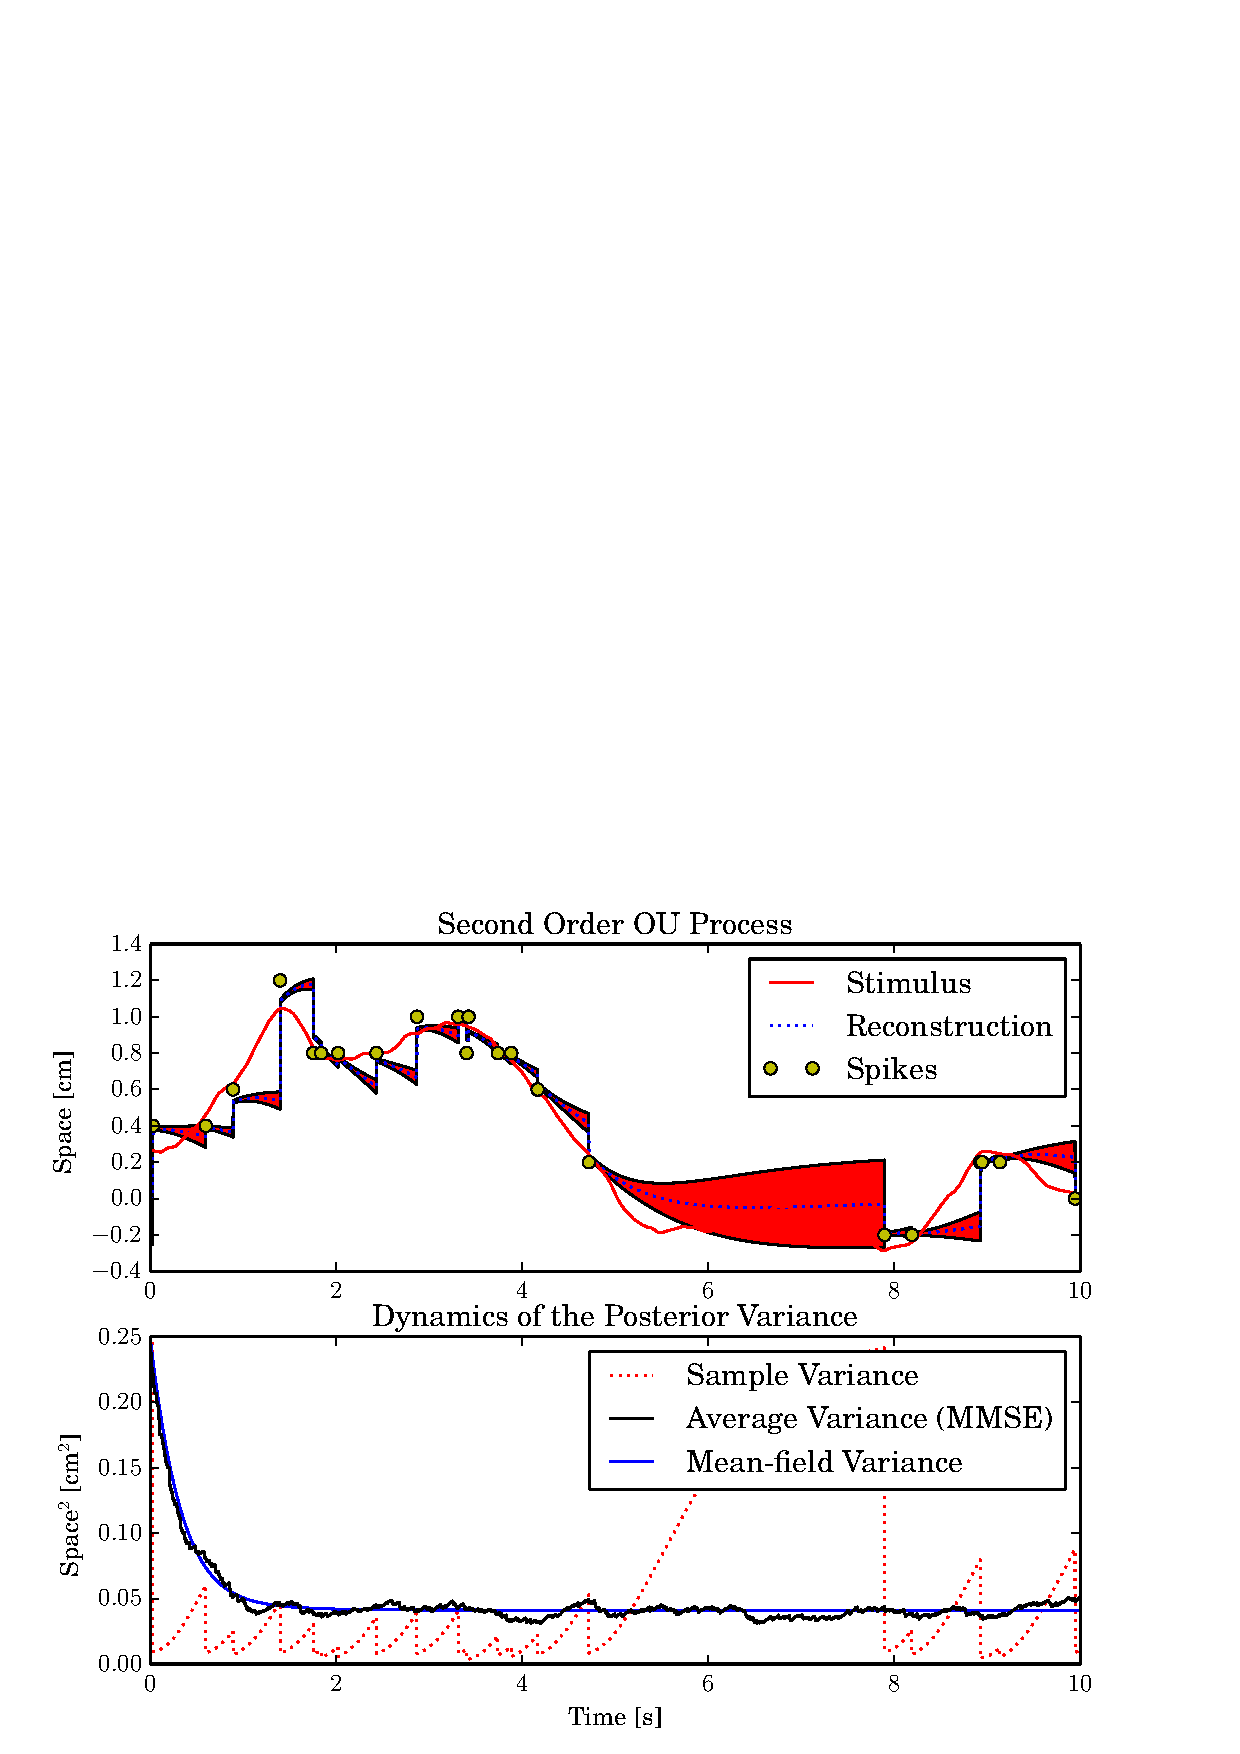
\includegraphics[width=\columnwidth]{figures/matern_coding.png}
\caption{THIS CAPTION MUST BE DONE!}
\end{figure}

We will now turn to filtering from Point processes when the dense coding assumption does not hold.

\section{Methods for General Filtering of Point Processes}

If nothing else is known about the process at hand, we are forced to work directly with \fref{eq:snyder_multi}. In principle one could discretize the state space and try to solve the Partial Differential Equation\marginnote{Partial Differential Equation $\equiv$ PDE} recursively as the observations come in. Note, however, that in truth the right hand side \fref{eq:snyder_multi} also contains averages over $P_t(x)$, leading to additional complications on every integration step. One way to circumvent this particular problem is to work with unnormalized probabilities. The Zakai equation\cite{Zakai1969} is a modified version of the Kushner equation which propagates unnormalized probabilities. Let us define $\rho_t(x)$, such that $P_t(x) = \rho_t(x)/\int dx \rho_t(x)$. Taking the same diffusion process notation as used in \fref{sec:kalman}, the evolution of $\rho_t(x)$ will be given by
\begin{equation}
\label{eq:zakai}
d\rho_t(x) = \mathcal{A} \rho_t(x) + \rho_t(x) x^\top c^\top \eta \eta^\top dz.
\end{equation}
Note that while the Kushner equation was a stochastic partial integro-differential equation, since the left hand side involved averages over $P_t(x)$, the Zakai equation is a simpler stochastic partial differential equation and given a realization of the observation process can be solved by standard methods. Furthermore, the Zakai equation allows for a closed form solution in terms of path integrals



